\begin{frame}{Variable transformations}
  \begin{itemize}
    \item Linear regression assumes linear relationships between independent and dependent variables
    \begin{itemize}
      \item i.e. a one-unit change in the independent variable associated with a constant change in the dependent variable
    \end{itemize}
    \item Sometimes we might think the effect is \emph{non-linear}
    \item To handle this, we \emph{transform} either the dependent or independent variables
  \end{itemize}
\end{frame}

\begin{frame}{Variable transformations: the logarithm}
  \begin{columns}
    \begin{column}{0.65\textwidth}
      \begin{itemize}
        \item The logarithm is a common variable transformation
        \item As the original variable gets larger, the change in the logarithm gets smaller
      \end{itemize}
    \end{column}~%
    \begin{column}{0.34\textwidth}
      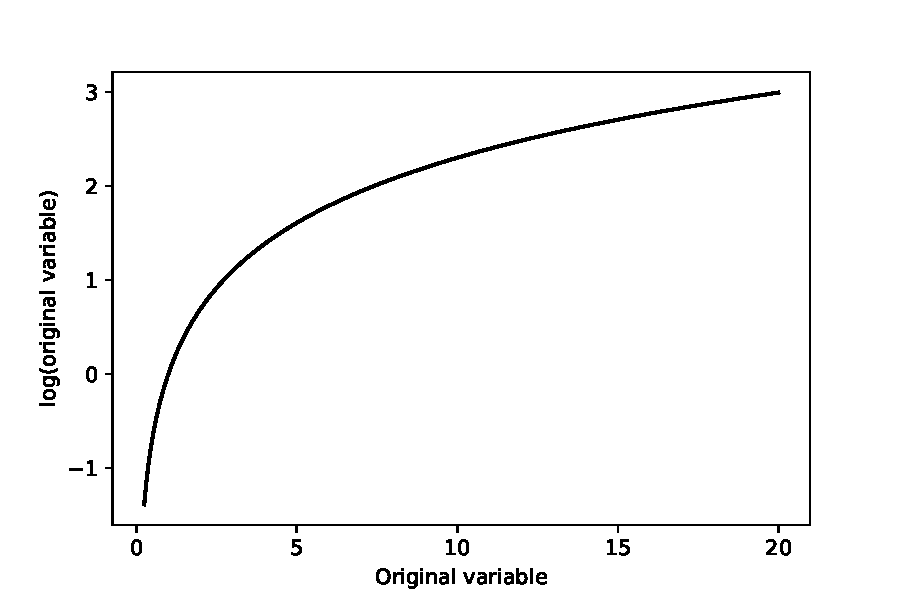
\includegraphics[width=\textwidth]{fig/log.pdf}
    \end{column}
  \end{columns}
\end{frame}

\begin{frame}{Variable transformations: logged dependent variable}
  \begin{columns}
    \begin{column}{0.65\textwidth}
      \begin{itemize}
        \item We log dependent variables when the effects of independent variables get larger at as the dependent variable does
        \item Maybe an additional bedroom is more valuable in a \$1,000,000 home than a \$100,000 home
        \item Coefficient interpretation: a one-unit increase in the independent variable is associated with an $100(e^\beta - 1)\%$ increase in the dependent variable \autocite{ford_interpreting_2018}
        \only<2>{\begin{itemize}
          \item when $\beta$ is small, $e^\beta - 1 \approx \beta$
        \end{itemize}}
      \end{itemize}
    \end{column}~%
    \begin{column}{0.34\textwidth}
      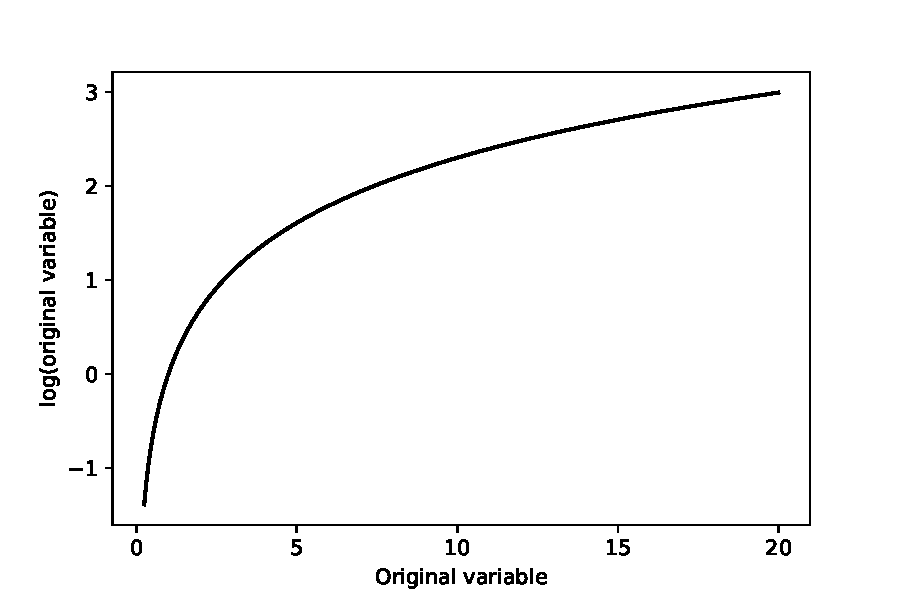
\includegraphics[width=\textwidth]{fig/log.pdf}
    \end{column}
  \end{columns}
\end{frame}


\begin{frame}{Variable transformations: logged independent variable}
  \begin{columns}
    \begin{column}{0.65\textwidth}
      \begin{itemize}
        \item We log independent variables when we think the association attenuates at larger values of the independent variable
        \item Maybe at high incomes, additional income matters less to driving, because people already go everywhere they want to
        \item Coefficient interpretation: a 1\% increase in the independent variable is associated with a $\frac{\beta}{100}$ absolute increase in the dependent variable \autocite{ford_interpreting_2018}
      \end{itemize}
    \end{column}~%
    \begin{column}{0.34\textwidth}
      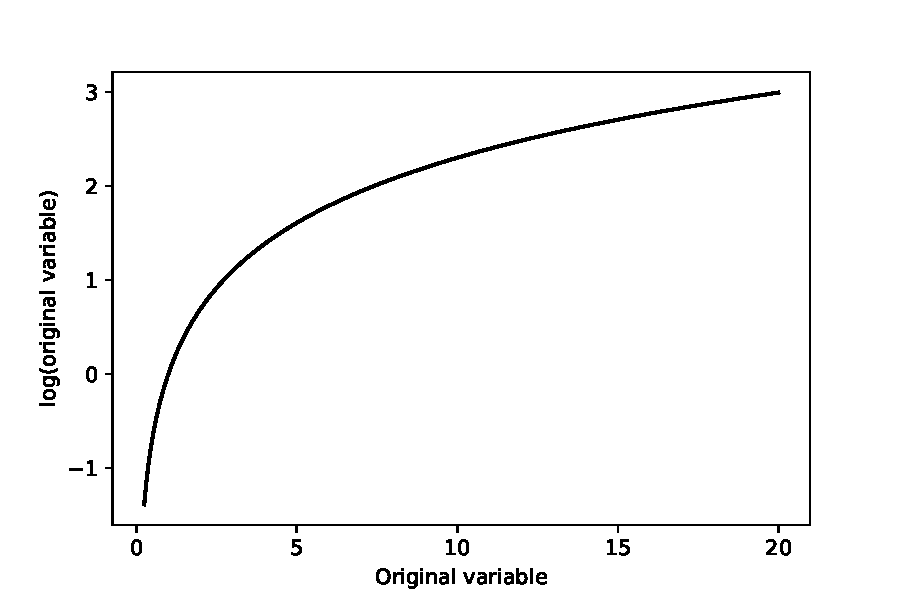
\includegraphics[width=\textwidth]{fig/log.pdf}
    \end{column}
  \end{columns}
\end{frame}

\begin{frame}{Variable transformations: logged dependent and independent variable}
  \begin{columns}
    \begin{column}{0.65\textwidth}
      \begin{itemize}
        \item We log dependent and independent variables when we think the relationship is multiplicative rather than additive
        \item The coefficient is then an \emph{elasticity}
        \item ...the percent change in the dependent variable for a 1\% change in the independent variable
      \end{itemize}
    \end{column}~%
    \begin{column}{0.34\textwidth}
      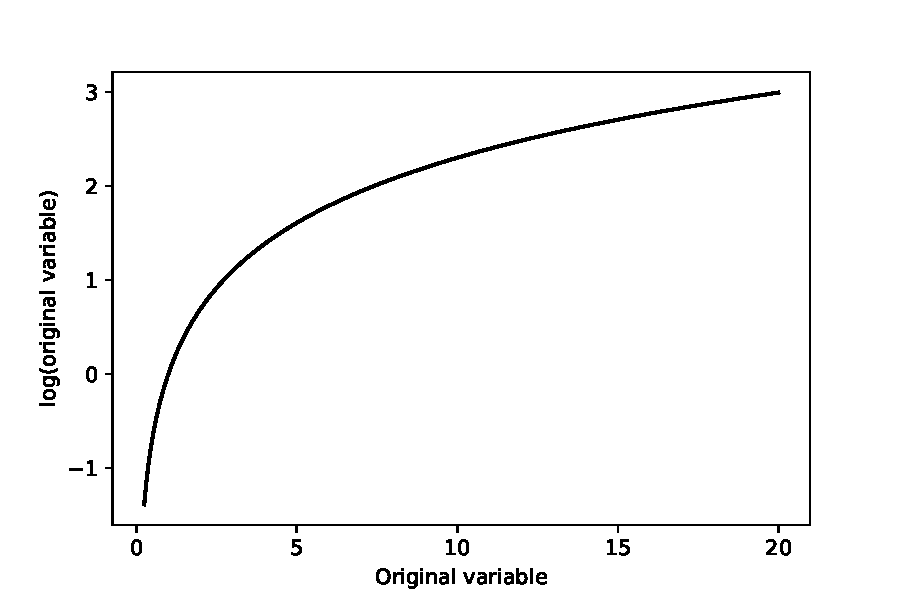
\includegraphics[width=\textwidth]{fig/log.pdf}
    \end{column}
  \end{columns}
\end{frame}

\begin{frame}{Other variable transformations}
  \begin{columns}
    \begin{column}{0.65\textwidth}
      \begin{itemize}
        \item {\color<1>{red}Power functions allow modelling U-shaped functions}
        \begin{itemize}
          \item {\color<2>{red}Powers beyond 2 are questionable}
        \end{itemize}
        \item {\color<3>{red}Piecewise regression allows different coefficient in different ranges}
        \item {\color<4>{red}Categorization estimates same value in each range}
      \end{itemize}
    \end{column}~%
    \begin{column}{0.34\textwidth}
      \only<1>{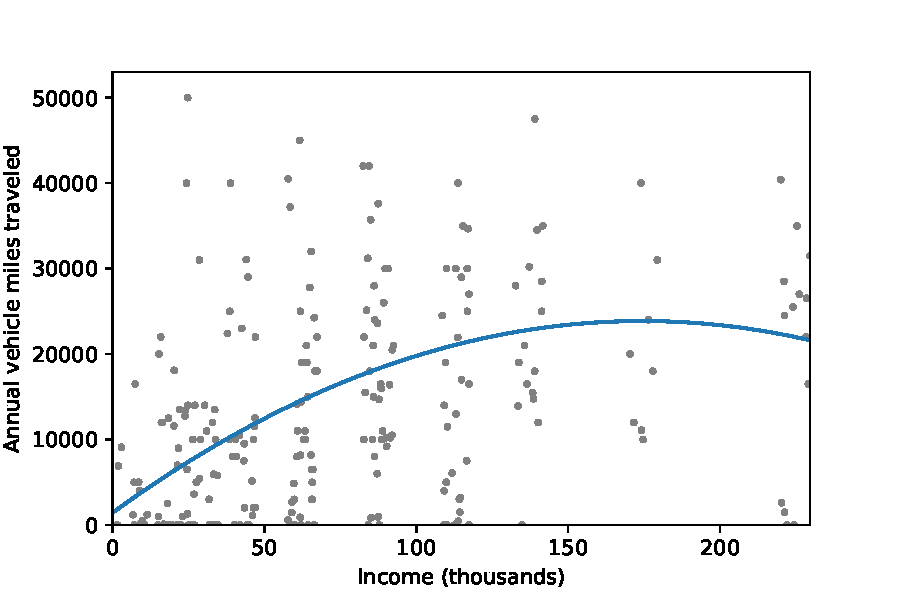
\includegraphics[width=\textwidth]{fig/power2.pdf}}
      \only<2>{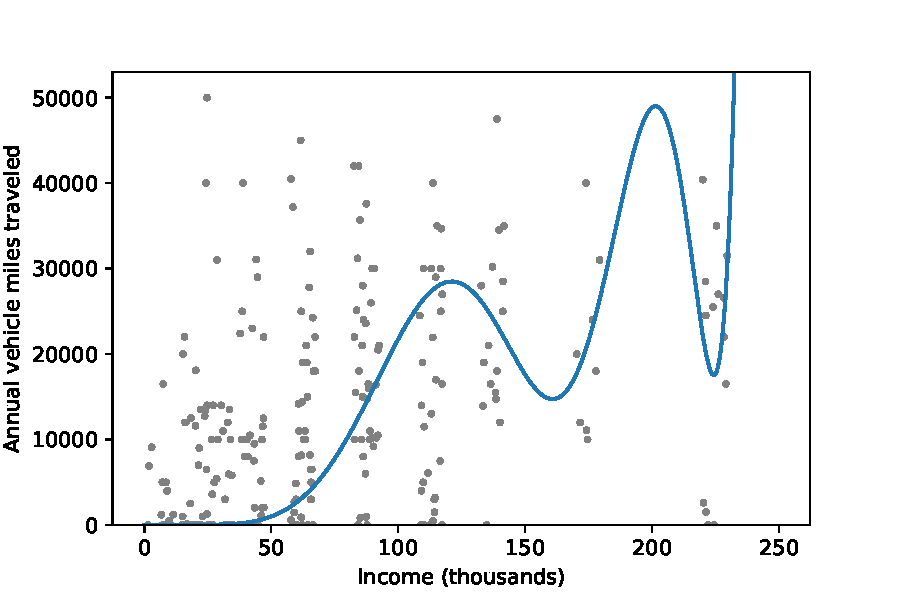
\includegraphics[width=\textwidth]{fig/overfitpower.pdf}}
      \only<3>{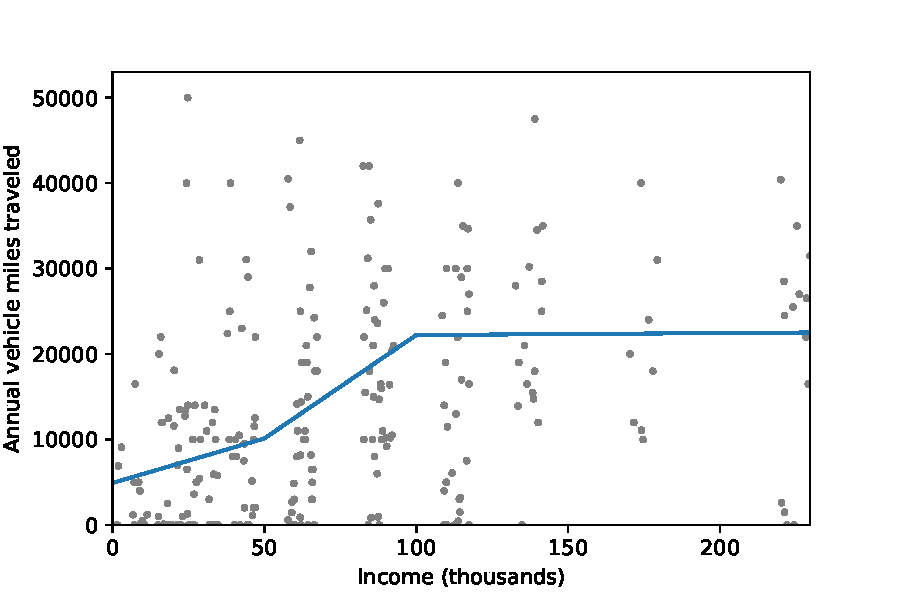
\includegraphics[width=\textwidth]{fig/piecewise.pdf}}
      \only<4>{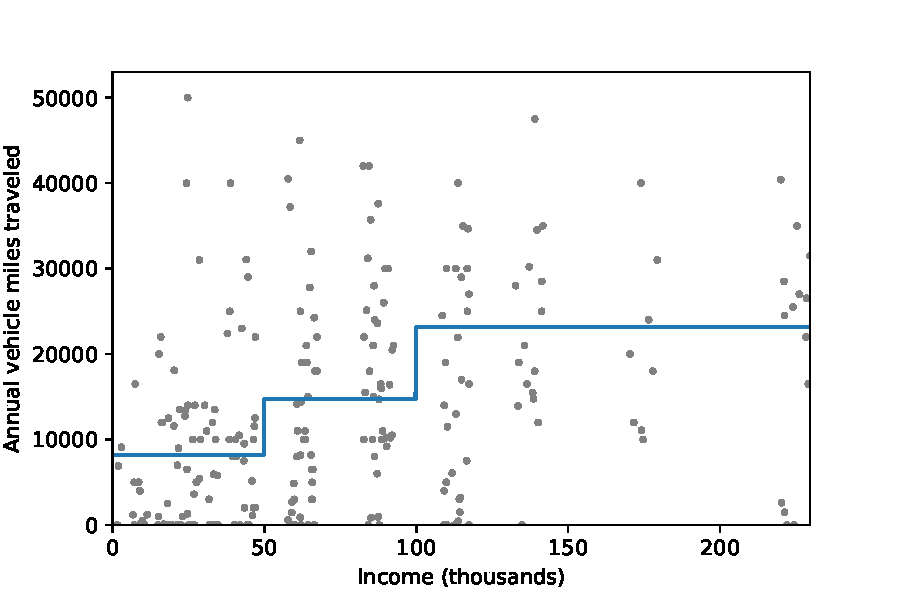
\includegraphics[width=\textwidth]{fig/categories.pdf}}
    \end{column}
  \end{columns}
\end{frame}

\begin{frame}{Interaction terms}
  \begin{itemize}
    \item What if we think the relationship between two variables is dependent on the value of a third variable?
    \item Maybe the effect of income differs across regions of the country
    \item We can use an \emph{interaction term}
    \item ...which means multiplying the two variables together
    \item Most often done with at least one dummy variable, easier to interpret
  \end{itemize}
\end{frame}

\begin{frame}{Interaction terms}
  \begin{equation*}
    \tikzmark{ydum} y = \alpha ~+~
    \beta_1\tikzmark{duminc}x_1 ~+~
    \beta_2\tikzmark{dumveh}x_2 ~+~
    \beta_3\tikzmark{dumrmw}x_3 ~+~
    \alt<3->{
      \textcolor{white}{\beta_4\tikzmark{dumrs}x_4}
    }{
      \textcolor{black}{\beta_4\tikzmark{dumrs}x_4}
    } ~+~
    \alt<4->{
      \textcolor{white}{\beta_5\tikzmark{dumrw}x_5}
    }{
      \textcolor{black}{\beta_5\tikzmark{dumrw}x_5}
    } ~+~
    \alt<5->{
      \textcolor{white}{\beta_6\tikzmark{sinc}x_4\tikzmark{incs}x_1}
    }{
      \textcolor{black}{\beta_6\tikzmark{sinc}x_4\tikzmark{incs}x_1}
    } ~+~
    \alt<6>{
      \textcolor{white}{\beta_7\tikzmark{winc}x_5\tikzmark{incw}x_1}
    }{
      \textcolor{black}{\beta_7\tikzmark{winc}x_5\tikzmark{incw}x_1}
    } ~+~
    \beta_8\tikzmark{mwinc}x_3\tikzmark{incmw}x_1 +
    \epsilon
  \end{equation*}

  \begin{tikzpicture}[overlay,remember picture]
    \draw[<-] ([xshift=0.5ex, yshift=1em] pic cs:ydum) -- +(90:0.1cm) -- +(70:0.7cm) node[anchor=south,text=black] { \scriptsize vehicle miles traveled } ;
    \draw[<-] ([xshift=0.8ex, yshift=1em] pic cs:dumveh) -- +(90:0.2cm) node[anchor=south,text=black] { \scriptsize number of vehicles } ;
    \draw[<-] ([xshift=0.8ex, yshift=1em] pic cs:dumrs) -- +(90:0.5cm) node[anchor=south,text=black] (slab) { \scriptsize South } ;

    \draw[<-] ([xshift=0.5ex, yshift=-0.1cm] pic cs:duminc) -- +(270:0.2cm) node[anchor=north,text=black] (inclab) { \scriptsize income (thousands) } ;
    \draw[<-] ([xshift=0.5ex, yshift=-0.1cm] pic cs:dumrmw) -- +(270:0.5cm) node[anchor=north,text=black] (mwlab) { \scriptsize Midwest } ;
    \draw[<-] ([xshift=0.5ex, yshift=-0.1cm] pic cs:dumrw) -- +(270:0.5cm) node[anchor=north,text=black] (wlab) { \scriptsize West } ;

    \draw[<-] ([xshift=0.5ex, yshift=-0.1cm] pic cs:winc) |- (wlab.east);
    \draw[<-] ([xshift=0.5ex, yshift=-0.1cm] pic cs:mwinc) -- +(270:1.5cm) -| (mwlab.south);
    \draw[<-] ([xshift=0.5ex, yshift=1em] pic cs:sinc) |- (slab.east);

    \draw[<-] ([xshift=0.5ex, yshift=-0.1cm] pic cs:incw) -- +(270:2.5cm) -| (inclab.south);
    \draw[<-] ([xshift=0.5ex, yshift=-0.1cm] pic cs:incmw) -- +(270:2.5cm) -| (inclab.south);
    \draw[<-] ([xshift=0.5ex, yshift=-0.1cm] pic cs:incs) -- +(270:2.5cm) -| (inclab.south);
  \end{tikzpicture}
  \pause

  \vspace*{2.75cm} What is the predicted VMT of a respondent in the Midwest?
\end{frame}

\begin{frame}{Interaction terms}
  \small
  \begin{tabular}{lrrrrrr}
\toprule
{} &  Coefficient &  Std. err. &  $t$-value &  $p$-value &  95\% Conf. &   Int. \\
\midrule
Constant           &        -2291 &       4649 &     -0.493 &      0.623 &     -11449 &   6867 \\
Income (thousands) &           74 &         50 &      1.484 &      0.139 &        -24 &    172 \\
Number of vehicles &         4393 &        903 &      4.867 &      0.000 &       2615 &   6170 \\
Region: Midwest    &        -4598 &       6167 &     -0.746 &      0.457 &     -16746 &   7550 \\
Region: South      &         3937 &       5019 &      0.784 &      0.434 &      -5950 &  13823 \\
Region: West       &         -235 &       5644 &     -0.042 &      0.967 &     -11353 &  10883 \\
Income (West)      &          -15 &         57 &     -0.255 &      0.799 &       -127 &     98 \\
Income (South)     &           17 &         55 &      0.313 &      0.755 &        -92 &    126 \\
Income (Midwest)   &           91 &         73 &      1.249 &      0.213 &        -53 &    235 \\
\bottomrule
\end{tabular}
\begin{tabular}{lclc}
Dependent variable & \multicolumn{3}{l}{Annual vehicle miles traveled} \\
$R^2$ & 0.24 & Adjusted $R^2$ & 0.21 \\
Sample size & 250 && \\
\end{tabular}\\
\tiny\citenhts
\end{frame}

% \begin{frame}{Interaction terms}
%   \begin{itemize}
%     \item What if we think that the relationship between two variables changes based on the value of another variable?
%     \item We can use an interaction term
%     \item An interaction term is the product of two independent variables
%     \item When both are large, it is large
%     \item When both are small, it is small
%     \item When either is small, it is in between
%     \item When the coefficient is positive, it means that when one of the independent variables is large, the effect of the other is more positive
%   \end{itemize}
% \end{frame}
%
% \begin{frame}{Interaction terms}
%   \small
%   \begin{tabular}{p{4cm}rrrrrr}
%   \toprule
%   {} &  Coefficient &  Std. err. &  $t$-value &  $p$-value &  95\% Conf. &  Int. \\
%   \midrule
%   Constant                                     &         -685 &       2563 &     -0.267 &      0.789 &      -5733 &  4362 \\
%   Income (thousands)                           &          120 &         23 &      5.295 &      0.000 &         75 &   164 \\
%   Number of vehicles                           &         3867 &        903 &      4.281 &      0.000 &       2088 &  5646 \\
%   Population density (thousands per sq. mi.)   &          326 &        351 &      0.927 &      0.355 &       -367 &  1018 \\
%   Interaction of income and population density &          -10 &          4 &     -2.565 &      0.011 &        -19 &    -2 \\
%   \bottomrule
%   \end{tabular}
%   \begin{tabular}{lclc}
%   Dependent variable & \multicolumn{3}{l}{Annual vehicle miles traveled} \\
%   $R^2$ & 0.23 & Adjusted $R^2$ & 0.22 \\
%   Sample size & 250 && \\
%   \end{tabular}
% \end{frame}

\begin{frame}{Pitfalls of linear regression: assumption of linearity}
  \begin{itemize}
    \item Linear regression assumes \emph{relationships are linear}
    \item Transformations can help
    \pause\item ...but not always clear which one to use
    \pause\item Best defense: \emph{does the model make sense?}
  \end{itemize}
\end{frame}

\begin{frame}{Pitfalls of regression: correlation does not imply causation}
  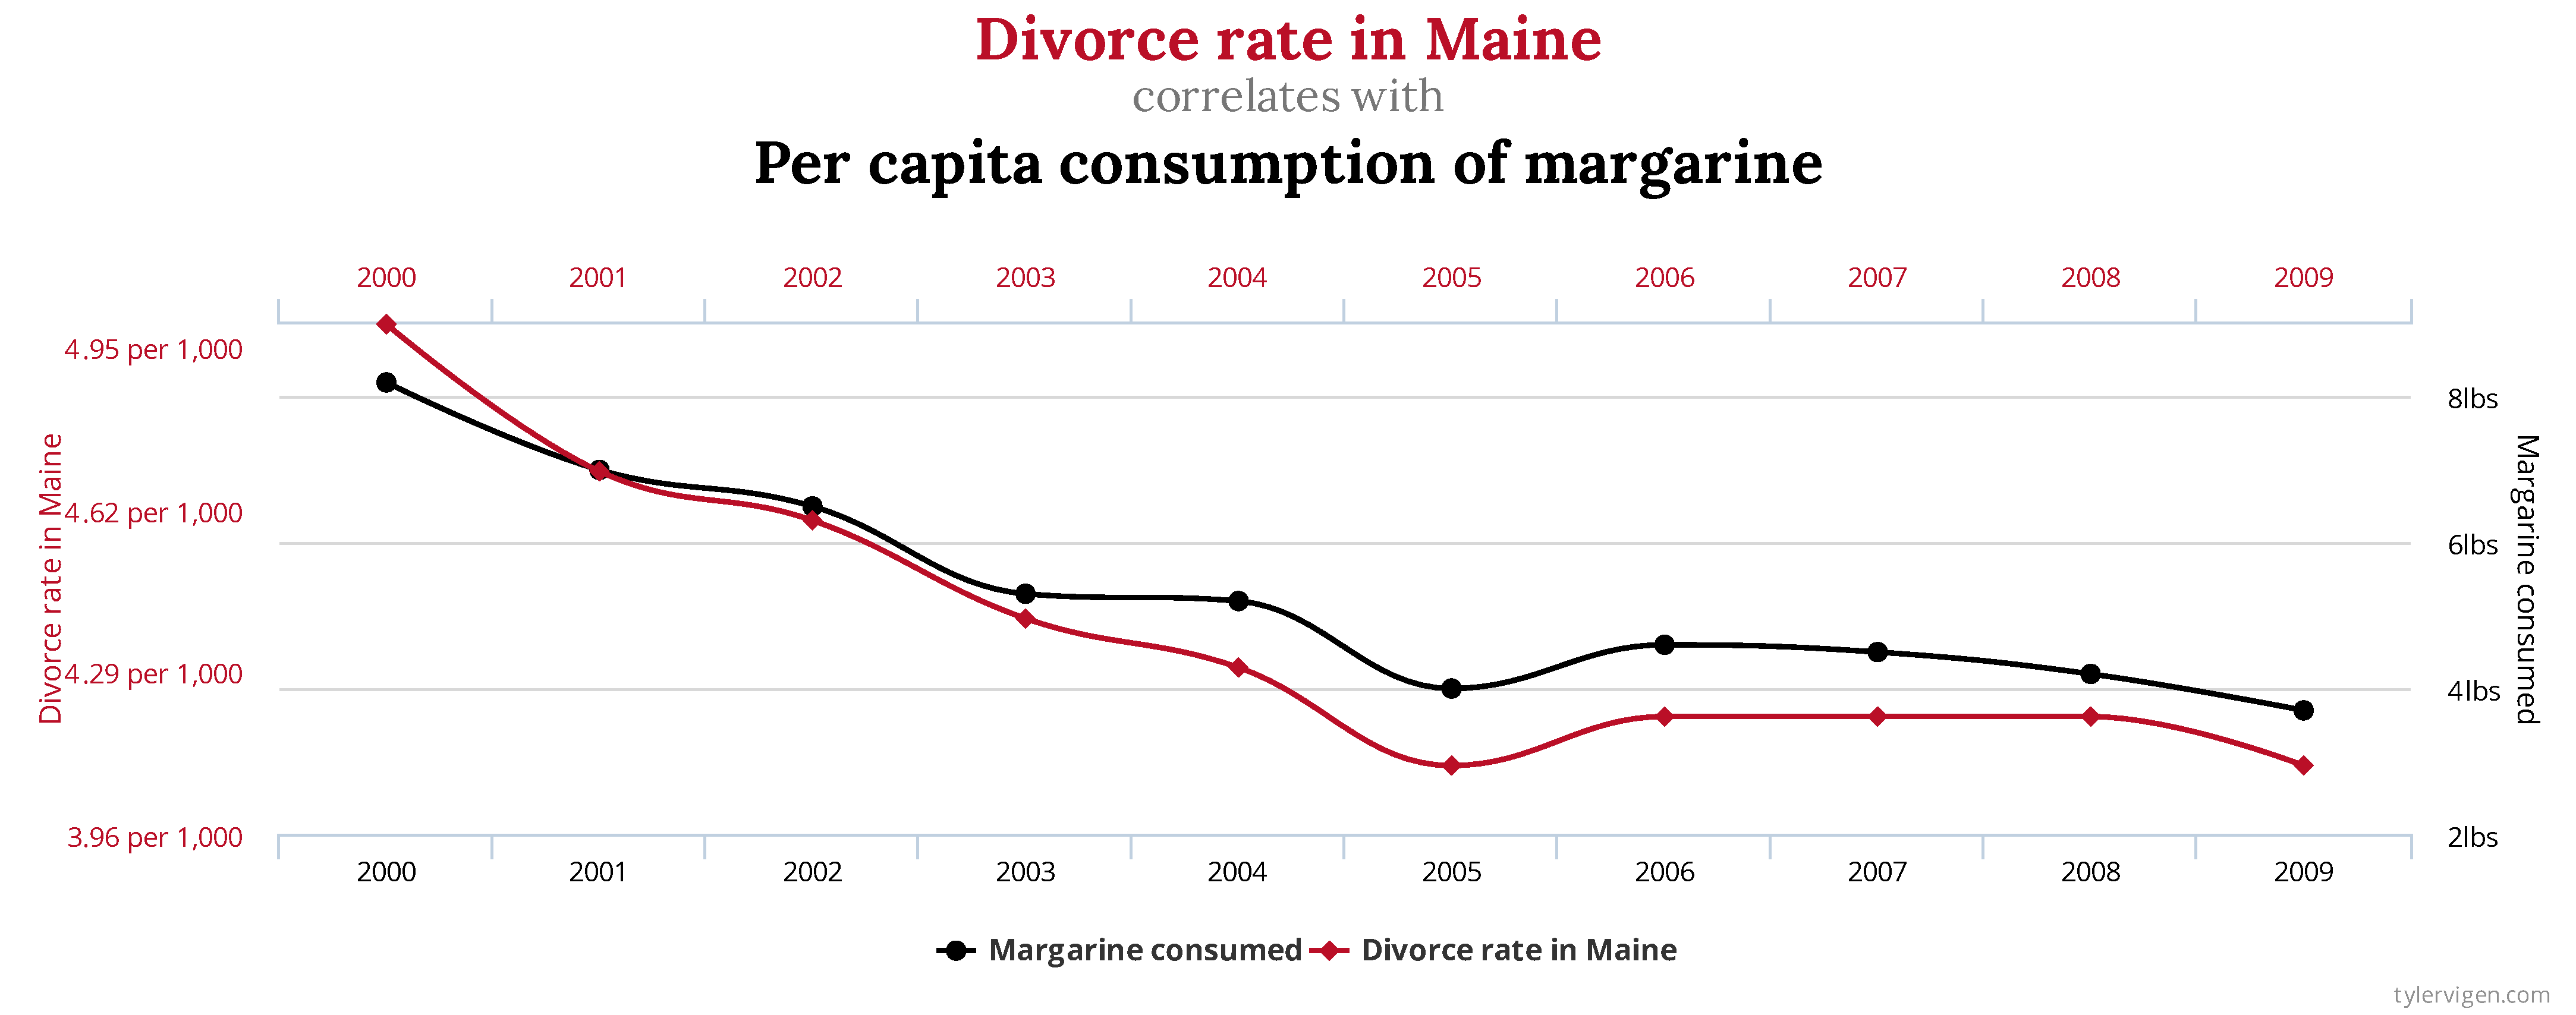
\includegraphics[width=\textwidth]{spurious_correlation.pdf}\\
  {\tiny \copyright~Tyler Vigen, tylervigen.com; CC BY 4.0}
\end{frame}

\begin{frame}{Pitfalls of regression: omitted variable bias}
  \begin{itemize}
    \item Every estimated association in the model depends on all the independent variables in the model
    \item If important variables are omitted, the remaining coefficients will be biased
    \item If we didn't have income in our model, the coefficient for number of vehicles would likely be larger
    \item ...because it would capture some of the income effect
    \pause\item Best defense: are there obvious variables \emph{missing from the model}?
  \end{itemize}
\end{frame}

\begin{frame}{Pitfalls of regression: multicollinearity}
  \begin{itemize}
    \item When variables are highly correlated, the regression cannot differentiate between them
    \item For example, population density and intersection density might be highly correlated
    \item The result is that the regression will not be able to determine which variable the independent variable is associated with, and both may become insignificant
  \end{itemize}
\end{frame}

\begin{frame}{Pitfalls of regression: multicollinearity}
  \begin{itemize}
    \item The usual diagnostic is the Variance Inflation Factor (VIF) for each coefficient
    \item Measured how much coefficient variance (square of the standard error) is increased due to multicollinearity
    \item Usual thresholds for concern are 4, 5 or 10, but depends on sample size and other factors \autocite[see][]{obrien_caution_2007}
  \end{itemize}
\end{frame}

\begin{frame}{Evaluating the fit of regression models: $R^2$}
  \begin{columns}
    \begin{column}{0.65\textwidth}
      \begin{itemize}
        \item proportion of variation in dependent variable explained by independent variables
        \item Ranges from 0--1
        \item Higher is better
      \end{itemize}
    \end{column}~%
    \begin{column}{0.34\textwidth}
      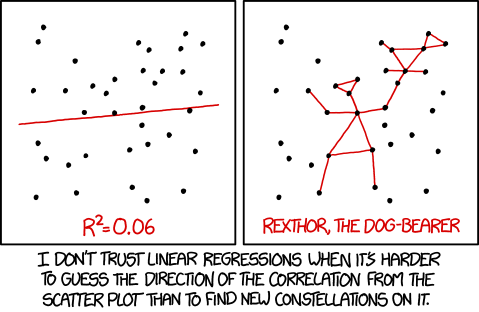
\includegraphics[width=\textwidth]{xkcd_linear_regression.png}
    \end{column}
  \end{columns}
\end{frame}

\begin{frame}{Evaluating the fit of regression models: Adjusted $R^2$}
  \begin{columns}
    \begin{column}{0.65\textwidth}
      \begin{itemize}
        \item Penalizes $R^2$ for the number of variables in the model
        \item When adding variables to a model, normal $R^2$ cannot go down
        \item But adjusted $R^2$ can
        \item Helps prevent \emph{overfitting}
      \end{itemize}
    \end{column}~%
    \begin{column}{0.34\textwidth}
      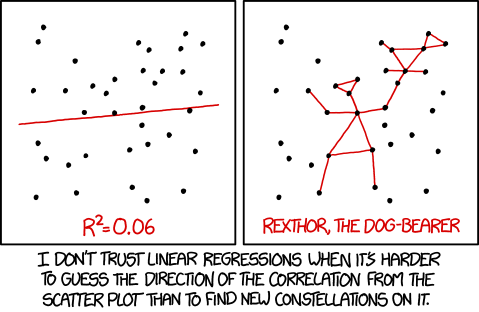
\includegraphics[width=\textwidth]{xkcd_linear_regression.png}\\
      {\tiny \copyright~xkcd, CC BY-NC 2.5}
    \end{column}
  \end{columns}
\end{frame}

\begin{frame}{Evaluating the fit of regression models: log-likelihood}
  \begin{itemize}
    \item The likelihood is the probability of observing the data given the coefficients
    \item Maximum likelihood estimation finds coefficients to maximize this probability
    \item Usually the logarithm of likelihood is used because it makes math easier
    \item Since probabilities range from 0--1, log-likelihoods range from $-\infty$--0
    \item Higher (closer to zero) is better
    \item Can't compare log-likelihoods of models with different dependent variables or samples
    \item A likelihood-ratio test is often used to determine if a more complex model is better than a nested simpler model
  \end{itemize}
\end{frame}

\begin{frame}{Evaluating the fit of regression models: log-likelihood}
  \begin{itemize}
    \item Authors may present up to three log-likelihood values
    \begin{itemize}
      \item Log-likelihood at convergence (may be notated LL($\beta$)): Log-likelihood of the full model with all coefficients
      \item Log-likelihood at constant(s) (LL(C)): Log-likelihood with only the constant in the model (or only the alternative specific constants in multinomial model)
      \item Log-likelihood at zero/null (LL(0)): Log-likelhood with all coefficients including the constant at zero
    \end{itemize}
    \item Models try to maximize LL($\beta$)
    \item The difference from LL(C) or LL(0) and LL($\beta$) is measure of how much better the model does than a model with no predictive power
  \end{itemize}
\end{frame}

\begin{frame}<1-3>{Evaluating the fit of regression models: AIC and BIC}
  \alt<2>{
    \centering \Large not to be confused with\\ \vspace{0.5cm}
    \begin{columns}
      \begin{column}{0.49\textwidth}
        \centering
\includegraphics[width=0.65\textwidth]{img/aoc.jpg}\\
        AOC
      \end{column}~%
      \begin{column}{0.5\textwidth}
        \centering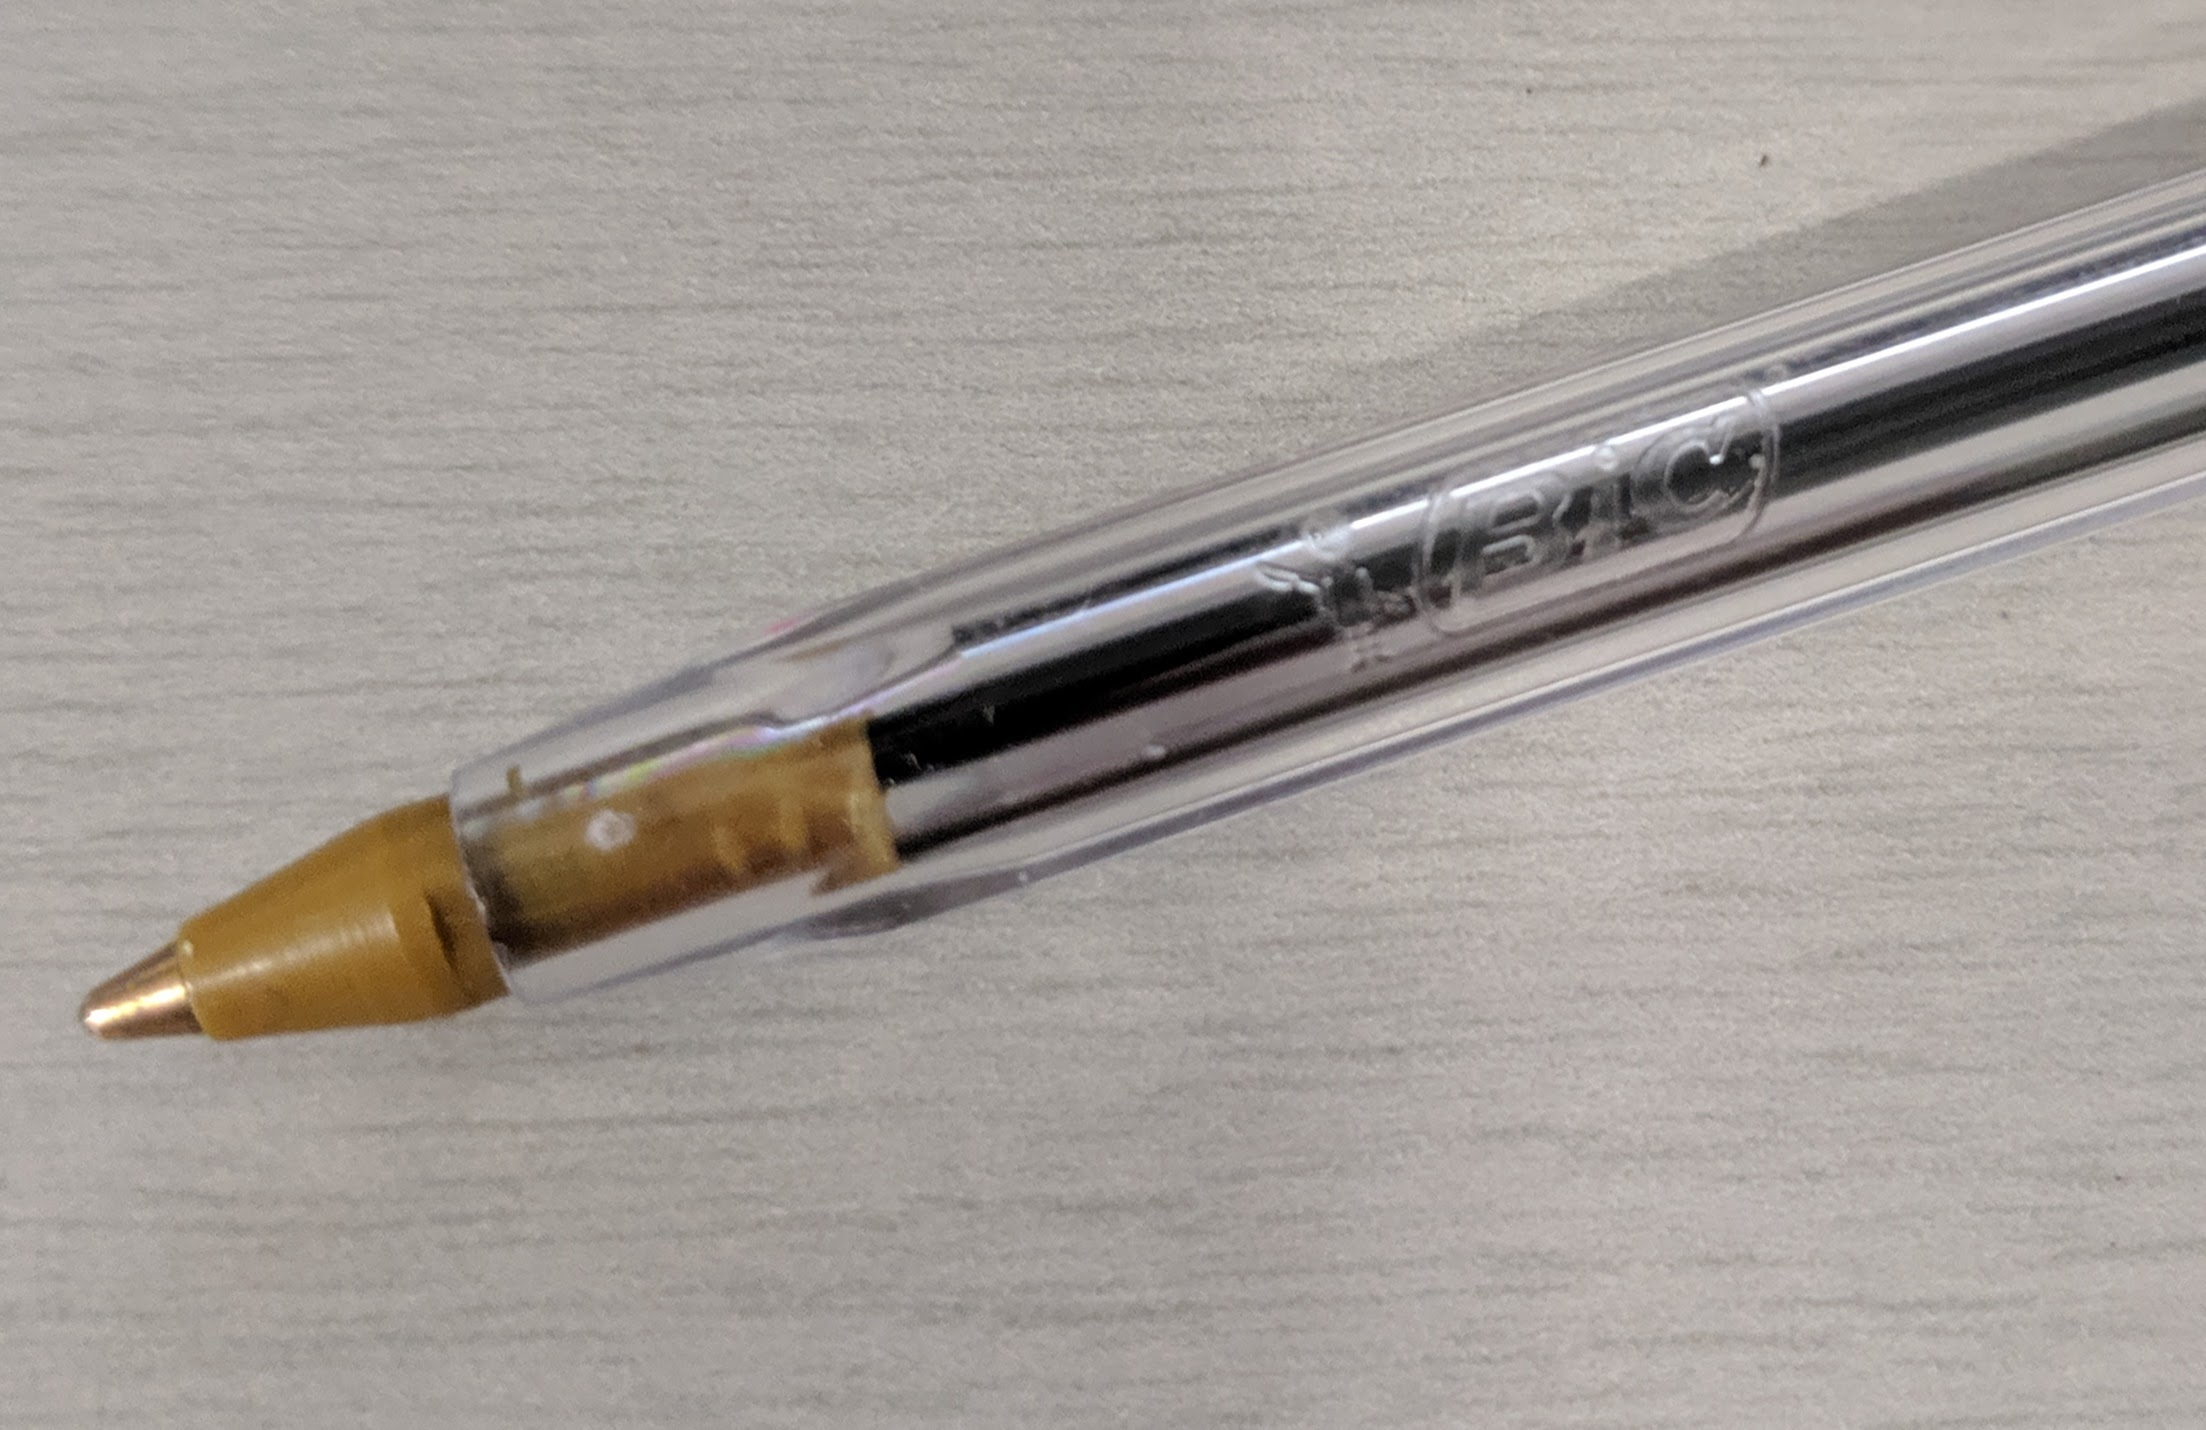
\includegraphics[width=\textwidth]{img/bic.jpg}\\
        Bic
      \end{column}
    \end{columns}
    }{
    \begin{itemize}
      \item Akaike Information Criterion (AIC) and Bayesian Information Criterion (BIC) also measure the fit of the model
      \item Transformations of the likelihood that penalize additional parameters, like Adjusted $R^2$
      \item Smaller values are better (unlike log-likelihood)
      \item Can't compare across different dependent variables or datasets
    \end{itemize}
  }
\end{frame}

\begin{frame}{Evaluating the fit of regression models: pseudo-$R^2$}
  \begin{itemize}
    \item Transformation of the log-likelihood function to make it behave ``more like'' an $R^2$
    \item Still can't be compared across different dependent variables or datasets \autocite{noauthor_faq_2011} % https://stats.idre.ucla.edu/other/mult-pkg/faq/general/faq-what-are-pseudo-r-squareds/
    \item Many types of pseudo-$R^2$'s available
  \end{itemize}
\end{frame}

\begin{frame}{Evaluating the fit of regression models: summary}
  \begin{tabular}{p{3cm}p{3cm}p{3cm}p{3cm}}
    \toprule
    \textbf{Measure} & \textbf{Higher or lower is better} & \textbf{Penalty for number of terms} & \textbf{    \raggedright\noindent Comparable across different data} \\
    \midrule
    $R^2$ & Higher is better & No & Yes \\
    Adjusted $R^2$ & Higher is better & Yes & Yes \\
    Log-likelihood & Higher (closer to zero) is better & No & No \\
    Akaike information criterion & Lower is better & Yes & No \\
    Bayesian information criterion & Lower is better & Yes & No \\
    pseudo-$R^2$ & Higher is better & Maybe & No \\
    \bottomrule
  \end{tabular}
\end{frame}

\begin{frame}{Evaluating the fit of regression models: why bother?}
  \begin{itemize}
    \item Goodness of fit is important if you want to \emph{predict} outcomes
    \item But when explaining relationships, it usually \emph{doesn't matter} very much
    \item Exception is when the predictive power is low because of omitted variables
  \end{itemize}
\end{frame}
